\subsection{Восстановление одиночного наследования}\label{chapter:full_sing_inhr_rec}
Как было сказано в главе \ref{chapter:info_extraction}, наследование на множестве классов $\gCa$ является одиночным. В случае использования только одиночного наследования, любое множество классов может быть представлено в виде нескольких деревьев наследования. Каждое дерево наследования является корневым деревом, причем ребра этого дерева заданы отношением непосредственного наследования.

В главе \ref{chapter:destructors} было отмечено, что для каждого класса $D$, принадлежащего некоторому дереву наследования, корнем которого является класс $B$, имеющий виртуальный деструктор, в результате применения утверждения \ref{stmt:destructors} будет получено ограничение $\cR_{\ref{stmt:destructors}}^{BD} = B \lhd D$. Таким образом, с использованием утверждения \ref{stmt:destructors} можно восстановить множество вершин любого дерева наследования с виртуальным деструктором, а таковых, как было отмечено в главе \ref{chapter:destructors}, большинство. В случае же отсутствия виртуального деструктора, множество вершин дерева наследования можно восстановить с использованием утверждения \ref{stmt:fsets}. Таким образом, множество $\gCa$ можно разбить на несколько непересекающихся подмножеств, каждое из которых будет задавать отдельное дерево наследования. С каждым из таких подмножеств можно работать отдельно, и поэтому, для упрощения дальнейших рассуждений, будем считать, что все классы из множества $\gCa$ принадлежат одному дереву наследования.

В этом случае восстановление иерархии классов подразумевает построение дерева наследования $T \in \nT^R(\gCa)$, а перечисленные выше источники информации о структуре иерархии определяют ограничения, которым это дерево должно удовлетворять. Пусть $\gR \subset \nT^R(\gCa) \rightarrow \{0, 1\}$ --- множество всех ограничений, полученных из утверждений \ref{stmt:vtable_size}, \ref{stmt:inherit_pure}, \ref{stmt:fsets_2}, \ref{stmt:param_size}, \ref{stmt:vcall} и \ref{stmt:destructors}, а $\gR_? \subset \nT^R(\gCa) \rightarrow \{0, 1\}$ --- множество всех ограничений, полученных из ненадежных источников информации, как это описано в главе \ref{chapter:unreliable}. В $\gR$ также входят ограничения, полученные из утверждений \ref{stmt:fsets_2} и \ref{stmt:vcall} в предположении о том, что дополнительные требования этих утверждений всегда выполнены. Это означает, что некоторые из ограничений из $\gR$ могут не выполняться.

Тогда задачу построения необходимого корневого дерева можно представить как задачу максимизации функции $\cF \in \nT^R(\gCa) \rightarrow \Rat \times \Rat$, определенной следующим образом:
\begin{equation}
\forall T \in \nT^R(\gCa): \cF(T) = (\sum_{\cR \in \gR} \cR(T), \sum_{\cR \in \gR_?} \cR(T))\text{,}
\end{equation}
где отношение $<$ на $\Rat \times \Rat$ определено следующим образом:
\begin{equation}
\forall (a_1, b_1), (a_2, b_2) \in \Rat \times \Rat: (a_1, b_1) < (a_2, b_2) \Longleftrightarrow a_1 < a_2 \vee (a_1 = a_2 \wedge b_1 < b_2)\text{.}
\end{equation}
Так как различные ограничения из $\gR_?$ могут иметь различную <<степень надежности>>, то при вычислении значения функции $\cF(T)$ возможно применение весовых коэффициентов.

При такой постановке задачи можно использовать ограничения произвольной формы, но при этом точное решение будет возможно получить лишь переборными методами. Приближенное же решение для задачи, поставленной в такой форме, можно получить, использовав метод генетического программирования. В работе \cite{palmer94} было предложено представление деревьев, которое дает хорошие результаты в применении к методам генетического программирования. Подобное представление может быть применено и для поставленной выше задачи.

Метод генетического программирования не всегда находит лучшее решение. С другой стороны, известно, что с большой вероятностью существует дерево наследования, удовлетворяющее всем ограничениям из $\gR$. Введем обозначение:
\begin{equation}
\begin{aligned}
& \isSol \in \nT^R(\gCa) \times 2^{\nT^R(\gCa) \rightarrow \{0, 1\}} \rightarrow \{0, 1\} \text{,}\\
& \forall T \in \nT^R(\gCa), \gR \in 2^{\nT^R(\gCa) \rightarrow \{0, 1\}}: \isSol(T, \gR) \Longleftrightarrow \forall \cR \in \gR: \cR(T)\text{.}
\end{aligned}
\end{equation}

Тогда, если не рассматривать ограничения из $\gR_?$, то в предположении, что все ограничения из $\gR$ могут быть выполнены, поставленная выше задача преобразуется в:
\begin{equation}\label{eq:problem}
\text{Найти~} T \in \nT^R(\gCa): \isSol(T, \gR)
\end{equation}

Так как возможна ситуация, что некоторые из ограничений из $\gR$ могут быть невыполнимы, и потому решения задачи \ref{eq:problem} может не существовать, необходимо построить алгоритм, который будет строить дерево наследования, удовлетворяющее как можно большему количеству ограничений из $\gR$, то есть множеству ограничений $\gR' \subseteq \gR$ такому, что:
\begin{equation}\label{eq:relaxed_gr}
\isSol(T, \gR') \wedge \forall \cR \in \gR \setminus \gR': \nexists T \in \nT^R(\gCa): \isSol(T, \gR' \cup \{\cR\})
\end{equation}

То есть представленный алгоритм должен решать следующую задачу:
\begin{equation}\label{eq:relaxed_problem}
\text{Найти~} \gR' \subseteq \gR, T \in \nT^R(\gCa): \text{~для $\gR'$ выполнено \ref{eq:relaxed_gr}}
\end{equation}



\subsubsection{Алгоритм построения частичного решения задачи восстановления одиночного наследования}\label{chapter:part_single_inher_rec}
Для каждой функции $f$ такой, что $\exists A \in \gCa, i \in \Nat: VT_A^i = f$ построим множество $\gf \subseteq \gCa: \forall C \in \gCa: C \in \gf \Longleftrightarrow VT_C^i = f$. Применяя к этому множеству утверждение \ref{stmt:fsets_2}, и учитывая то, что все ограничения, порожденные этим утверждением, принадлежат множеству $\gR$, получаем:
\begin{equation}\label{eq:is_sol_req}
\forall T \in \nT^R(\gCa): \isSol(T, \gR) \Longrightarrow T[\nT][\gf] \in \nT(\gf) \text{,}
\end{equation}
то есть для того, чтобы дерево $T$ являлось решением задачи (\ref{eq:problem}), необходимо, чтобы его сужение на множество $\gf$ также являлось деревом. Пусть $\gF$ --- множество всех таких множеств $\gf$. Введем обозначение:
\begin{equation}\label{eq:is_partial_solution}
\begin{aligned}
& \isPartSol \in \nT(\gCa) \times 2^{2^{\gCa}} \rightarrow \{0, 1\} \text{,}\\
& \forall T \in \nT(\gCa), \gF \in 2^{2^{\gCa}}: \isPartSol(T, \gF) \Longleftrightarrow \forall \gf \in \gF: T[\gf] \in \nT(\gf)\text{.}
\end{aligned}
\end{equation}

Из (\ref{eq:is_sol_req}) и (\ref{eq:is_partial_solution}) следует:
\begin{equation}\label{eq:is_sol_req_2}
\forall T \in \nT^R(\gCa): \isSol(T, \gR) \Longrightarrow \isPartSol(T[\nT], \gF) \text{,}
\end{equation}
то есть $\isPartSol(T[\nT], \gF)$ является необходимым условием того, что дерево $T$ является решением задачи (\ref{eq:problem}). Будем говорить, что если выполнено $\isPartSol(T[\nT], \gF)$, то дерево $T$ является частичным решением задачи (\ref{eq:problem}).

Пусть
\begin{equation}\label{eq:f_closure_def}
\gFc = \bigcup_{\gF' \subseteq \gF} \left\{ \bigcap_{\gf \in \gF'} \gf \right\} \text{,}
\end{equation}
то есть $\gF^{\cap}$ --- множество всевозможных пересечений множеств из $\gF$. Оценим количество элементов в множестве $\gFc$. Для этого сначала докажем следующую лемму:



\vspace{1cm}
\begin{lemma}\label{lemma:tree_subdivision}
Для любого конечного множества $X$, в любом дереве $T \in \nT(X)$ можно выбрать вершину $x \in X$ таким образом, что при удалении этой вершины и всех инцидентных ей ребер из дерева $T$, это дерево распадется на несколько деревьев, в каждом из которых будет не более $\left\lfloor\frac{|X|}{2}\right\rfloor$ вершин.
\end{lemma}
\begin{proof}
Пусть для некоторого дерева $T$ такую вершину выбрать нельзя, то есть для любой вершины $x \in X$ при ее удалении из дерева $T$, это дерево распадается на несколько поддеревьев, в одном из которых содержится более $\left\lfloor\frac{|X|}{2}\right\rfloor$ вершин. Таких поддеревьев не может быть два, так как иначе в них суммарно содержалось бы более $|X|$ вершин. Обозначим множество вершин такого поддерева, соответствующего вершине $x$, через $V_x$. В множестве $V_x$ содержится ровно одна вершина, инцидентная $x$ в дереве $T$. Обозначим эту вершину $x'$. Тогда возможны два варианта:

\begin{figure}[htb!]
\centering
\begin{minipage}[b]{6cm}
\centering
\includegraphics[scale=1.0]{images/tree_division.png}
\caption{Вариант $x \notin V_{x'}$.}
\label{fig:tree_division}
\end{minipage}
\hspace{0.5cm}
\begin{minipage}[b]{6cm}
\centering
\includegraphics[scale=1.0]{images/tree_division_2.png}
\caption{Вариант $x \in V_{x'}$.}
\label{fig:tree_division_2}
\end{minipage}
\end{figure}

\begin{enumerate}
\item $x \notin V_{x'}$, рис. \ref{fig:tree_division}. В этом случае можно взять $x = x'$ и повторить приведенные выше рассуждения. В силу конечности множества $V_{x'}$, когда-нибудь будет верно, что:
\item $x \in V_{x'}$, рис. \ref{fig:tree_division_2}. В этом случае $V_{x'} \cap V_x = \emptyset$, и $|V_{x'}| + |V_x| > |X|$, что невозможно.
\end{enumerate}
Полученное противоречие завершает доказательство леммы.
\end{proof}
\vspace{1cm}



С использованием леммы \ref{lemma:tree_subdivision} оценим количество элементов в множестве $\gFc$.



\vspace{1cm}
\begin{lemma}\label{lemma:f_closure_size}
Если $k$ --- максимальное количество функций в таблицах виртуальных функций классов из некоторого множества классов $\gC$, $\gF \subseteq 2^{\gC}$, $n = |\gC|$, и $\exists T \in \nT(\gC): \isPartSol(T, \gF)$, то $|\gFc| \le 2n^{k + \log_2{3}}$.
\end{lemma}
\begin{proof}
%Для каждого класса из $\gC$ определено не более $k$ виртуальных функций, и поэтому каждый класс может принадлежать не более чем $k$ различным множествам из $\gF$. Это в частности означает, что:
%\begin{equation}\label{eq:gf_size}
%|\gF| \le nk
%\end{equation}

Пусть $\psi(\gF) = |\gFc|$, а $\nF_k(\gC) \subseteq 2^{2^{\gC}}$ --- множество всевозможных $\gF \subseteq 2^{\gC}$ таких, что каждый элемент из $\gC$ принадлежит не более чем $k$ различным множествам из $\gF$, и $\exists T \in \nT(\gC): \isPartSol(T, \gF)$. Тогда определим функцию $\phi$ следующим образом:
\begin{equation}\label{eq:phi_definition}
\phi(n, k) = \max_{\gF \in \nF_k(\gC) \wedge |\gC| = n} \psi(\gF) \text{.}
\end{equation}

Для функции $\phi$ выполнено:
\begin{equation}\label{eq:phi_additive}
\phi(n_1, k) + \phi(n_2, k) \le \phi(n_1 + n_2, k)\text{.}
\end{equation}

Действительно, для любых двух множеств
\begin{equation}
\begin{aligned}
\gF_1 &\in \nF_k(\gC_1): |\gC_1| = n_1 \text{,} \\
\gF_2 &\in \nF_k(\gC_2): |\gC_2| = n_2 \wedge \gC_1 \cap \gC_2 = \emptyset \text{,}
\end{aligned}
\end{equation}
и деревьев
\begin{equation}\label{eq:t1_t2_def}
\begin{aligned}
T_1 &\in \nT(\gC_1): \isPartSol(T_1, \gF_1) \text{,} \\
T_2 &\in \nT(\gC_2): \isPartSol(T_2, \gF_2) \text{,}
\end{aligned}
\end{equation}
можно взять $T$ --- дерево, полученное из деревьев $T_1$ и $T_2$ добавлением ребра, соединяющего вершину $A$ дерева $T_1$ с вершиной $C$ дерева $T_2$, и $\gF = \gF_1 \cup \gF_2 \cup \{A, C\}$. В силу $\gC_1 \cap \gC_2 = \emptyset$, выполнено $\gF_1 \cap \gF_2 = \emptyset$, и потому единственным общим элементом множеств $\gFc_1$ и $\gFc_2$ может быть пустое множество. Так как $\gFc_1 \in \gFc$ и $\gFc_2 \in \gFc$, и возможное наличие общего элемента в $\gFc_1$ и $\gFc_2$ скомпенсировано наличием элемента $\{A, C\}$ в $\gFc$, отсутствующего в $\gFc_1$ и $\gFc_2$, то будет справедливо $|\gFc_1| + |\gFc_2| \le |\gFc|$.

В силу \ref{eq:t1_t2_def} и \ref{eq:is_partial_solution}, по построению для $T$ будет выполнено $\isPartSol(T, \gF)$. Следовательно, $\gFc \in \nF_k(\gC_1 \cup \gC_2)$, и поэтому, согласно (\ref{eq:phi_definition}):
\begin{equation}
\psi(\gF_1) + \psi(\gF_2) \le \psi(\gF) \le \phi(n_1 + n_2, k) \text{.}
\end{equation}

В силу того, что $\gF_1$ и $\gF_2$ были выбраны произвольно из множеств $\nF_k(\gC_1)$ и $\nF_k(\gC_2)$ соответственно, выполнено и неравенство (\ref{eq:phi_additive}). Из этого неравенства также следует то, что функция $\phi(n, k)$ является неубывающей по $n$.

Рассмотрим некоторые фиксированные множество $\gF$ и соответствующее ему дерево $T$ такие, что $\isPartSol(T, \gF)$. В силу леммы \ref{lemma:tree_subdivision}, в этом дереве можно выделить вершину $A$ так, что при удалении этой вершины и всех инцидентных ей ребер это дерево распадется на несколько деревьев $T_i$, каждое из которых будет состоять не более, чем из $\left\lfloor\frac{n}{2}\right\rfloor$ вершин. Пусть $m$ --- количество деревьев, на которые распалось дерево $T$, $\gF_i$ --- подмножество $\gF$, элементы которого целиком лежат в множестве вершин $T_i$, а $\gF_A$ --- подмножество $\gF$, элементы которого содержат $A$. В силу того, что элементы любых двух множеств $\gF_i$ не пересекаются, выполнено неравенство:
\begin{equation}\label{eq:psi_decomp}
\psi(\gF) \le \psi(\gF_A) \sum_{i = 1}^{m} \psi(\gF_i)\text{.}
\end{equation}

Так как $A$ принадлежит не более чем $k$ множествам из $\gF$, всевозможных пересечений которых не более чем $2^k$, то в силу (\ref{eq:f_closure_def}) выполнено $\psi(\gF_A) = |\gFc_A| \le 2^k$, и неравенство (\ref{eq:psi_decomp}) преобразуется в:
\begin{equation}\label{eq:psi_decomp_2}
\psi(\gF) \le 2^k \sum_{i = 1}^{m} \psi(\gF_i)\text{.}
\end{equation}

Пусть $n_i$ --- количество вершин в $i$-м дереве. Тогда полученные $m$ деревьев можно разделить на три группы так, как это показано на рисунке \ref{fig:three_division}. При этом в каждой группе будет суммарно не более $\left\lfloor\frac{n}{2}\right\rfloor$ вершин.

\begin{figure}[htb!]
\centering
\includegraphics[scale=1.0]{images/three_division.png}
\caption{Разбиение множества деревьев $\{T_i\}$ на три группы, в каждой из которых суммарно не более $\left\lfloor\frac{n}{2}\right\rfloor$ вершин.}
\label{fig:three_division}
\end{figure}

Тогда неравенство (\ref{eq:psi_decomp_2}) преобразуется в:
\begin{equation}\label{eq:psi_decomp_3}
\begin{aligned}
\psi(\gF) &\le 2^k \sum_{i = 1}^{m} \psi(\gF_i) \\
&= 2^k \left( \sum_{i = 1}^{l-1} \psi(\gF_i) + \psi(\gF_l) + \sum_{i = l+1}^{m} \psi(\gF_i) \right) \\
&\le 2^k \left( \sum_{i = 1}^{l-1} \phi(n_i, k) + \phi(n_l, k) + \sum_{i = l+1}^{m} \phi(n_i, k) \right) \\
&\{\text{согласно (\ref{eq:phi_additive})} \} \\
&\le 2^k \left( \phi(\sum_{i = 1}^{l-1} n_i, k) + \phi(n_l, k) + \phi(\sum_{i = l+1}^{m} n_i, k) \right) \\
&\{\text{$\phi$ --- неубывает по $n$}\}\\
&\le 3 \cdot 2^k \phi(\left\lfloor\frac{n}{2}\right\rfloor, k) \text{.}
\end{aligned}
\end{equation}

Так как $\phi(1, k) = 2$, то согласно (\ref{eq:psi_decomp_3}), для функции $\phi$ справедлива следующая оценка:
\begin{equation}
\phi(n, k) \le 2 \cdot 2^{k \log_2{n}}3^{\log_2{n}} = 2n^{k + \log_2{3}}\text{,}
\end{equation}
что завершает доказательство леммы.
\end{proof}
\vspace{1cm}



Полученное неравенство дает верхнюю оценку размера множества $\gFc$. В результате проведения экспериментов было выяснено, что в задачах, встречающихся на практике, размер множества $\gFc$ в большинстве случаев не превышает $n^2$.

Для множества $\gFc$ выполнена следующая лемма.

\vspace{1cm}
\begin{lemma}\label{lemma:f_closure_tree}
Для произвольного множества классов $\gC$ выполнено $\forall T \in \nT(\gC), \gF \subseteq 2^{\gC}: \isPartSol(T, \gF) \Longrightarrow \isPartSol(T, \gFc)$.
\end{lemma}
\begin{proof}
Пусть утверждение леммы не верно. Тогда, согласно (\ref{eq:is_partial_solution}), $\exists~\gf':~T[\gf'] \notin \nT(\gf')$. Множество $\gf'$ не может быть пустым, потому как сужение дерева на пустое множество является деревом, и не может содержать только одну вершину, так как сужение дерева на множество из одной вершины также всегда является деревом. Следовательно, в множестве $\gf'$ содержится минимум две вершины.

В $T[\gf']$ не может быть циклов, так как их нет в $T$, и при сужении не добавляются новые ребра. Следовательно, $T[\gf']$ может не быть деревом только если оно не связно. Не нарушая общности, будем считать, что в $T[\gf']$ --- две компоненты связности. Пусть вершина $A$ лежит в первой компоненте, а $B$ --- во второй. По определению множества $\gFc$, $\gf'$ было получено пересечением некоторого количества множеств из $\gF$, то есть:
\begin{equation}
\gf' = \bigcap_{\gf \in \gF'} \gf \text{,}
\end{equation}
где $\gF' \subseteq \gF$. Значит, вершины $A$ и $B$ принадлежат всем множествам из $\gF'$. Так как по условию леммы $\forall \gf \in \gF': T[\gf] \in \nT(\gf)$, то если бы в $T$ между $A$ и $B$ существовал только один простой путь, то он принадлежал бы всем деревьям $T[\gf]$, где $\gf \in \gF'$, и, следовательно, все вершины этого простого пути принадлежали бы пересечению множеств из $\gF'$, и потому этот простой путь также принадлежал бы дереву $T[\gf']$, что противоречит предположению об отсутствии пути между вершинами $A$ и $B$ в $T[\gf']$. Следовательно, в $T$ существует несколько простых путей между $A$ и $B$. Но $T$ --- это дерево, и потому в нем существует единственный простой путь между вершинами $A$ и $B$. Полученное противоречие завершает доказательство леммы.
\end{proof}
\vspace{1cm}



Рассмотрим множество $\gFs$, определенное следующим образом:
\begin{equation}\label{eq:gfs_def}
\gFs = \gFc \cup \{\gCa\} \cup \bigcup_{C \in \gCa}\{\{C\}\} \setminus \emptyset \text{.}
\end{equation}

В силу того, что $T[\gCa] = T$, и сужение любого дерева на множество из одного элемента также является деревом, выполнено:
\begin{equation}\label{eq:gfs_tree}
\isPartSol(T, \gFc) \Longleftrightarrow \isPartSol(T, \gFs) \text{.}
\end{equation}

По построению также выполнено, что любое пересечение множеств из $\gFs$ содержится в $\gFs$. Тогда из (\ref{eq:is_sol_req_2}), (\ref{eq:gfs_tree}) и леммы \ref{lemma:f_closure_tree} следует:
\begin{equation}\label{eq:is_sol_req_3}
\forall T \in \nT^R(\gCa): \isSol(T. \gR) \Longrightarrow \isPartSol(T[\nT], \gFs) \text{,}
\end{equation}
то есть $\isPartSol(T[\nT], \gFs)$ является необходимым условием того, что дерево $T$ является решением задачи (\ref{eq:problem}).

Рассмотрим отношение $\subset$ на множестве $\gFs$. Это отношение является отношением частичного порядка, и поэтому для него можно построить диаграмму Хассе.

Диаграмма Хассе\footnote{англ. Hasse diagram.} --- графическое представление частично упорядоченного множества $(X, \le)$, в котором с каждым элементом $X$ сопоставляется точка плоскости таким образом, что меньшая точка всегда располагается ниже большей точки. Две точки $x$ и $y$ в диаграмме Хассе соединены тогда и только тогда, когда $x \le y$, и не существует такой точки $z$, что $x \le z \le y$.

Пусть диаграмма Хассе $\gH = (\gFs, \subset)$ для множества $\gFs$ построена. Каждой вершине $\gH$ соответствует множество из $\gFs$. Будем обозначать вершины $\gH$ также, как и элементы множества $\gFs$, то есть если $\gf \in \gFs$, то будем говорить, что $\gf$ является вершиной $\gH$. В силу (\ref{eq:is_sol_req_3}), если дерево $T$ является решением задачи (\ref{eq:problem}), то каждой вершине $\gf$ диаграммы Хассе $\gH$ соответствует поддерево $T[\gf]$ дерева $T$.

Диаграмму Хассе $\gH$ можно рассматривать как неориентированный граф. Будем обозначать множество ребер этого графа $\gH_E$.

Рассмотрим алгоритм построения дерева $T$ такого, что выполнено $\isPartSol(T, \gFs)$, представленный на рис. \ref{alg:build_tree}.

\begin{figure}[htb!]
\begin{algorithmic}[1]
\STATE $T_E = \emptyset$
\FORALL{$\gf \in \gFs$}
    \STATE $\gD \gets \{\gf' \in \gFs | \gf' \subset \gf \wedge \{\gf, \gf'\} \in \gH_E\}$
    \STATE $\gK \gets \gD$
    \WHILE{$\exists \gf_1, \gf_2 \in \gK: \gf_1 \cap \gf_2 \ne \emptyset$}
        \STATE $\gK \gets \gK \setminus \{\gf_1, \gf_2\} \cup \{\gf_1 \cup \gf_2\}$
    \ENDWHILE
    \STATE $t \gets any(\nT(\gK))$
    \FORALL{$\{\gf_1, \gf_2\} \in t_E$}
        \STATE $T_E \gets T_E \cup \{any(\gf_1), any(\gf_2)\}$
    \ENDFOR
\ENDFOR
\RETURN $T = (\gCa, T_E)$
\end{algorithmic}
\caption{Алгоритм построения дерева $T$ по множеству $\gFs$.}
\label{alg:build_tree}
\end{figure}

Представленный на рис. \ref{alg:build_tree} алгоритм использует функцию $any$, которая возвращает произвольный элемент данного множества. Для этого алгоритма справедлива следующая теорема.



\vspace{1cm}
\begin{theorem}\label{theorem:evil}
Если $\exists T' \in \nT(\gCa): \isPartSol(T', \gFs)$, то алгоритм, представленный на рис. \ref{alg:build_tree}, строит дерево $T \in \nT(\gCa): \isPartSol(T, \gFs)$ независимо от того, какие значения были возвращены функциями $any$.
\end{theorem}
\begin{proof}
Покажем, что в результате применения алгоритма будет выполнено $\forall \gf \in \gFs: T[\gf] \in \nT(\gf)$. Так как $\gCa \in \gFs$, то из этого будет следовать справедливость теоремы.

Будем рассматривать вершины диаграммы Хассе $\gH$ в порядке снизу вверх. Такой порядок просмотра гарантирует, что при рассмотрения очередного множества $\gf \in \gFs$, все множества $\gf' \in \gFs: \gf' \subset \gf$ будут уже рассмотрены. Пронумеруем элементы множества $\gFs$ в соответствии с этим порядком: $\gFs = \{\gf_1, \gf_2, \ldots, \gf_{|\gFs|}\}$. В этом случае будет справедливо
\begin{equation}\label{eq:seq_prop}
\gf_i \subset \gf_j \Longrightarrow i < j \text{.}
\end{equation}

Пусть
\begin{equation}\label{eq:induct}
\forall \gf_i: 1 \le i \le n - 1: T[\gf_i] \in \nT(\gf_i) \text{,}
\end{equation}
где $1 \le n \le |\gFs|$. Покажем, что в этом случае будет выполнено и $T[\gf_n] \in \nT(\gf_n)$.

В случае, если $\gf_n$ состоит из одной вершины, $T[\gf_n]$ является деревом.

Рассмотрим случай $|\gf_n| > 1$. В процессе выполнения алгоритма к $\gf_n$ было применено тело основного цикла. В результате было построено соответствующее $\gf_n$ множество $\gD$. Согласно определению множества $\gD$, в нем содержатся все вершины диаграммы Хассе $\gH$, находящиеся ниже $\gf_n$, и соединенные с $\gf_n$ ребром. Так как $|\gf_n| > 1$, то согласно (\ref{eq:gfs_def}), выполнено $\forall C \in \gf_n: \{C\} \in \gFs$, и потому множество $\gD$ не пусто.

Рассмотрим множество $\gK$, построение которого происходит в строках 4-7 алгоритма. По построению выполнено:
\begin{equation}\label{eq:gk_props}
\begin{aligned}
&\forall \gf'_1, \gf'_2 \in \gK: \gf'_1 \ne \gf'_2 \Longrightarrow \gf'_1 \cap \gf'_2 = \emptyset \\
&\gf_n = \bigcup_{\gf' \in \gK} \gf'
\end{aligned}
\end{equation}

В строках 8-11 над множеством $\gK$ строится произвольное дерево, и в соответствии со структурой этого дерева добавляются ребра к дереву $T$. Заметим, что если выполнено $\forall \gf' \in \gK: T[\gf'] \in \nT(\gf')$, то будет также выполнено и $T[\gf_n] \in \nT(\gf_n)$. Действительно, если над каждым из множеств из $\gK$ уже построено дерево, то в силу (\ref{eq:gk_props}), в результате добавления ребер в строках 8-11 алгоритма $T[\gf_n]$ будет связным графом с $\sum_{\gf' \in \gK} |\gf'|$ вершин и $\sum_{\gf' \in \gK} (|\gf'| - 1) + |\gK| - 1 = \sum_{\gf' \in \gK} |\gf'| - 1$ ребер, то есть деревом.

Покажем, что для всех $\gf' \in \gK$, $T[\gf']$ является деревом. Проведем доказательство для некоторого отдельного множества $\gf' \in \gK$. По построению, каждый элемент множества $\gK$ является объединением некоторого количества элементов множества $\gD$, то есть:
\begin{equation}\label{eq:gft_is_gc_gft_union}
\gf' = \bigcup_{\gf \in \gD} \gf \text{,}
\end{equation}
где $\gD \subseteq \gD$. Так как для всех $\gf \in \gD$ выполнено $\gf \subset \gf_n$, то в силу (\ref{eq:seq_prop}) и (\ref{eq:induct}), также выполнено:
\begin{equation}\label{eq:all_in_gc_are_trees}
\forall \gf \in \gD: T[\gf_i] \in \nT(\gf_i) \text{.}
\end{equation}

Из (\ref{eq:gft_is_gc_gft_union}) и (\ref{eq:all_in_gc_are_trees}) следует, что $\forall \gf \in \gD: T[\gf_i] \in \nT(\gf_i)$. То есть $T[\gf']$ является <<объединением>> некоторого количества деревьев, причем граф $T[\gf']$ связен. Покажем, что $T[\gf']$ --- дерево.

Пусть это не так. Так как граф $T[\gf']$ связен, и не является деревом, то в нем должен присутствовать один или несколько простых циклов, то есть циклов, в которых вершины и ребра не повторяются.

Пусть отношение $\subseteq$ на множестве неориентированных графов над некоторым множеством $X$ определено как $\forall G = (G_V, G_E), G' = (G'_V, G'_E) \in \nG(X): G \subseteq G' \Longleftrightarrow G_V \subseteq G'_V \wedge G_E \subseteq G'_E$, то есть $G$ является подграфом $G'$. Тогда зададим отношение $\subset$: $\forall G, G' \in \nG(X): G \subset G' \Longleftrightarrow G \subseteq G' \wedge G \ne G'$. Аналогично вводятся операции $\cup$ и $\cap$ над множеством $\nG(X)$.

Рассмотрим некоторый простой цикл $S \subseteq T[\gf']$. Тогда для любого $\gf \in \gD$ пересечение $S \cap T[\gf]$ пусто или состоит из одного или нескольких отрезков из $S$. Каждый такой отрезок может быть рассмотрен как простой путь в $S$, то есть путь, в котором вершины и ребра не повторяются. Пусть $\gS_{\gf}$ --- множество таких отрезков для $\gf$. По построению для этого множества выполнено:
\begin{equation}\label{eq:gs_for_gf_def}
\forall_{\gs \in \gS_{\gf}, \gs' \subseteq S \cap T[\gf]} \; \text{$\gs'$ --- отрезок} \Longrightarrow \gs \cap \gs' = \emptyset \vee \gs' \subseteq \gs
\end{equation}

Будем считать, что каждый отрезок из $\gS_{\gf}$ помечен множеством $\gf$. Пусть $\gS$ является объединением всех таких множеств $\gS_{\gf}$, то есть:
\begin{equation}
\gS = \bigcup_{\gf \in \gD} \gS_{\gf} \text{.}
\end{equation}

По построению для $\gS$ выполнено:
\begin{equation}
\bigcup_{\gs \in \gS} \gs = S
\end{equation}

Так как каждый отрезок из $\gS$ помечен множеством из $\gD$, то пусть функция $\cI$ для каждого отрезка возвращает соответствующее ему множество из $\gD$.

Заметим, что если $\exists \gs_i, \gs_j \in \gS: \cI(\gs_i) = \cI(\gs_j)$, то между некоторыми двумя вершинами отрезков $\gs_i$ и $\gs_j$ существует простой путь $\gp_{ij}$ в $T[\cI(\gs_i)]$. Соответствующий пример представлен на рис. \ref{fig:two_same_segment}. Этот путь не может целиком лежать в $S$, так как тогда было бы нарушено (\ref{eq:gs_for_gf_def}) --- пересечение $T[\cI(\gs_i)]$ с $S$ состояло бы из одного или нескольких отрезков, одним из которых являлся бы $\gs_i \cup \gp_{ij} \cup \gs_j$, и потому отрезки $\gs_i$ и $\gs_j$ не попали бы в множество $\gS_{\cI(\gs_i)}$.

\begin{figure}[htb!]
\centering
\begin{minipage}[t]{0.4\textwidth}
\centering
\includegraphics[scale=1.0]{images/two_same_segment.png}
\caption{Пример существования в простом цикле нескольких отрезков, которым соответствует одно и то же множество.}
\label{fig:two_same_segment}
\end{minipage}
\hspace{0.5cm}
\begin{minipage}[t]{0.4\textwidth}
\centering
\includegraphics[scale=1.0]{images/two_same_segment_2.png}
\caption{Результат обработки случая, представленного на рис. \ref{fig:two_same_segment}.}
\label{fig:two_same_segment_2}
\end{minipage}
\end{figure}

Таким образом, между некоторыми двумя вершинами, лежащими на отрезках $\gs_i$ и $\gs_j$, существуют два простых пути --- один лежащий в $S$, другой --- лежащий в $\gp_{ij}$, причем ни один из этих простых путей не содержится в другом. Но тогда это означает, что в графе, построенном путем объединения этих двух простых путей, существует простой цикл. Обозначим этот цикл $S^{(1)}$. Пусть $\gs^{(1)} = (\gs_i \cup \gp_{ij} \cup \gs_j) \cap S^{(1)}$, тогда простой цикл $S^{(1)}$ можно покрыть множеством отрезков:
\begin{equation}\label{eq:gs_1_def}
\gS^{(1)} \subseteq \gS \cup \{\gs^{(1)}\} \setminus \{\gs_i, \gs_j\}
\end{equation}

Будем считать, что $\gS^{(1)}$ выбрано так, что все отрезки из $\gS^{(1)}$ имеют непустое пересечение с $S^{(1)}$. Так как в процессе построения структура цикла была изменена, то для некоторых отрезков из $\gS^{(1)}$ может больше не выполняться (\ref{eq:gs_for_gf_def}), примененное к циклу $S^{(1)}$, то есть не обязательно выполняется:
\begin{equation}\label{eq:gs_for_gf_def_2}
\forall_{\gs \in \gS^{(1)}, \gs' \subseteq S^{(1)} \cap T[\cI(\gs)]} \; \text{$\gs'$ --- отрезок} \Longrightarrow \gs \cap \gs' = \emptyset \vee \gs' \subseteq \gs
\end{equation}

Заменим каждый отрезок $\gs \in \gS^{(1)}$ на $\gs_+$ такой, что для $\gs_+$ выполняется (\ref{eq:gs_for_gf_def_2}), и при этом $\gs \cap \gs_+ \ne \emptyset$. Полученное таким образом новое множество отрезков обозначим $\gS^{(1)}_+$. Будем считать, что если в результате замены в $\gS^{(1)}_+$ были добавлены два равных отрезка, которым соответствует одно и то же множество из $\gD$, то такие отрезки представлены в множестве $\gS^{(1)}_+$ только один раз. Так как множество $\gS^{(1)}$ покрывало цикл $S^{(1)}$, то и построенное множество $\gS^{(1)}_+$ будет его покрывать.

Заметим, что в силу (\ref{eq:gs_1_def}), выполнено $|\gS^{(1)}| < |\gS|$, и потому также выполнено $|\gS^{(1)}_+| < |\gS|$. Так как количество отрезков в множестве $\gS$ конечно, то повторяя несколько раз приведенные выше рассуждения, на $k$-м шаге будет выполнено $\nexists \gs_i, \gs_j \in \gS^{(k)}_+: \cI(\gs_i) = \cI(\gs_j)$.

Выделим минимальное подмножество отрезков $\gS_{\min} \subseteq \gS^{(k)}_+$, покрывающих весь простой цикл $S^{(k)}$, то есть:
\begin{equation}\label{eq:gsmin_def}
\begin{aligned}
\bigcup_{\gs \in \gS_{\min}} \gs &= S^{(k)} \\
\forall \gs' \in \gS_{\min} \bigcup_{\gs \in \gS_{\min} \setminus \{\gs'\}} \gs &\ne S^{(k)}
\end{aligned}
\end{equation}

\begin{figure}[htb!]
\centering
\begin{minipage}[t]{0.4\textwidth}
\centering
\includegraphics[scale=1.0]{images/two_segment.png}
\caption{Пример отрезка, лежащего целиком внутри другого отрезка.}
\label{fig:two_segments}
\end{minipage}
\hspace{0.5cm}
\begin{minipage}[t]{0.4\textwidth}
\centering
\includegraphics[scale=1.0]{images/three_segment.png}
\caption{Пример пересечения отрезков кратности три.}
\label{fig:three_segments}
\end{minipage}
\end{figure}

Для этого подмножества выполнено:
\begin{itemize}
\item В $\gS_{\min}$ нет отрезков, целиком лежащих внутри других. Если $\exists \gs_1, \gs_2 \in \gS_{\min}: \gs_1 \subseteq \gs_2$, то $\gS'_{\min} = \gS_{\min} \setminus \{\gs_1\}$ также покрывает весь простой цикл $S^{(k)}$, что противоречит определению множества $\gS_{\min}$. Пример для данного случая представлен на рис. \ref{fig:two_segments}.
\item Среди пересечений отрезков из $\gS_{\min}$ нет пересечений кратности три. На рис. \ref{fig:three_segments} представлен пример пересечения кратности три. Как видно, отрезок $\gs_1$ не может содержаться в $\gS_{\min}$, так как отрезки $\gs_2$ и $\gs_3$ и так покрывают соответствующие $\gs_1$ вершины и ребра. В общем случае, если существует пересечение кратности три, то среди отрезков, его образующих, существует отрезок $\gs_1$ такой, что $\gs_1 \subseteq \gs_2 \cup \gs_3$, где $\gs_2$ и $\gs_3$ --- два оставшихся отрезка в этом пересечении. Тогда $\gS'_{\min} = \gS_{\min} \setminus \{\gs_1\}$ также покрывает весь простой цикл $S^{(k)}$, что противоречит определению множества $\gS_{\min}$.
\end{itemize}

Таким образом, среди пересечений отрезков из $\gS_{\min}$ существуют только пересечения кратности два, и простой цикл $S^{(k)}$ можно представить как последовательность отрезков $S^{(k)} = (\gs_1, \ldots, \gs_n)$, в которой только соседние отрезки имеют непустое пересечение. Выбрав по точке на каждом пересечении соседних отрезков, получим последовательность точек $(C_1, \ldots, C_n)$ такую, что любые две соседние точки $C_i$ и $C_{i + 1}$ лежат в отрезке $\gs_i$, и потому лежат и в $\cI(\gs_i)$.

По условию теоремы, $\exists T' \in \nT(\gCa): \isPartSol(T', \gFs)$, то есть сужение дерева $T'$ на любое множество из $\gFs$ является деревом. Тогда сужение $T'$ на любое из множеств $\cI(\gs_i)$ также является деревом, и потому в каждом из таких деревьев существует единственный простой путь между соответствующими вершинами $C_i$ и $C_{i + 1}$. Обозначим этот простой путь $\gp_i$. По построению эти простые пути образуют цикл $S_{T'} = (\gp_1, \ldots, \gp_n)$. Так как $T'$ является деревом, то этот цикл не может быть простым, и каждая вершина из этого цикла принадлежит как минимум двум простым путям. Это означает, что в этом цикле существуют два простых пути $\gp_i$ и $\gp_{i+1}$, образующих <<поворот>>, как это изображено на рис. \ref{fig:tree_turn}.

\begin{figure}[htb!]
\centering
\includegraphics[scale=1.0]{images/tree_turn.png}
\caption{Пример <<поворота>>, образованного двумя простыми путями в цикле, не являющимся простым.}
\label{fig:tree_turn}
\end{figure}

Но тогда один из простых путей $\gp_i$ и $\gp_{i+1}$ содержится в другом. Не нарушая общности, будем считать, что $\gp_i$ содержится в $\gp_{i+1}$. Это означает, что $C_i$ содержится в $\gp_{i + 1}$, и так как по построению множество вершин простого пути $\gp_{i + 1}$ является подмножеством $\cI(\gs_{i + 1})$, то $C_i \in \cI(\gs_{i + 1})$.

Вернемся к дереву $T$. По построению для $\cI(\gs_{i + 1})$ выполнено $C_{i + 1}, C_{i + 2} \in \cI(\gs_{i + 1})$. $T[\cI(\gs_{i + 1})]$ является деревом, и поэтому в нем существует единственный простой путь из $C_i$ в $C_{i + 1}$, и единственный простой путь из $C_{i + 1}$ в $C_{i + 2}$. Эти простые пути должны принадлежать циклу $S^{(k)}$, и потому в силу (\ref{eq:gs_for_gf_def_2}) они также должны принадлежать отрезку $\gs_{i + 1}$. Но тогда среди отрезков из $\gS_{\min}$ существует пересечение кратности три --- $C_i \in \gs_{i + 1}$, $C_i \in \gs_{i}$, $C_i \in \gs_{i - 1}$, что противоречит определению множества $\gS_{\min}$. Следовательно, изначальное предположение о том, что в $T[\gf']$ существует цикл, неверно, и $T[\gf']$ является деревом. 

Полученное противоречие доказывает, что если выполнено (\ref{eq:induct}), то выполнено и $T[\gf_n] \in \nT(\gf_n)$. Тогда применение метода математической индукции для индукционного перехода (\ref{eq:induct}) и для базы индукции $n = 1$, дает, что (\ref{eq:induct}) верно для всех $1 \le n \le |\gFs|$, что завершает доказательство теоремы.
\end{proof}
\vspace{1cm}



Следствием доказанной теоремы является то, что любое решение задачи (\ref{eq:problem}) может быть получено с помощью алгоритма \ref{alg:build_tree}, а также то, что если в результате применение алгоритма \ref{alg:build_tree} не было построено дерево, то невозможно одновременно удовлетворить все ограничения вида $\cR_{\ref{stmt:fsets_2}}$, порожденные утверждениями \ref{stmt:fsets_2}. В этом случае путем автоматического анализа имеющейся информации затруднительно выяснить, какое из ограничений вида $\cR_{\ref{stmt:fsets_2}}$ следует удалить из множества $\gR$. Поэтому будем считать, что в этом случае удаление вызывающего конфликт ограничения выполняется вручную. Как было отмечено в комментарии к утверждению \ref{stmt:fsets_2}, такая ситуация маловероятна. В дальнейшем будем считать, что все ограничения, порожденные утверждением \ref{stmt:fsets_2}, выполнены. Для этого случая модифицируем алгоритм \ref{alg:build_tree} так, чтобы он строил только решения задачи (\ref{eq:relaxed_problem}).











\subsubsection{Алгоритм построения решения задачи восстановления одиночного наследования}\label{chapter:restore_single_inheritance}
Рассмотрим диаграмму Хассе $\gH$. Алгоритм \ref{alg:build_tree} для каждой вершины $\gf$ этой диаграммы строит множество $\gD$. Будем называть элементы этого множества дочерними вершинами для $\gf$ в диаграмме Хассе $\gH$. По диаграмме Хассе $\gH$ построим граф $\gG$, вершинами которого также являются множества $\gf \subset \gCa$, но разделенные на два типа --- $\any$ и $\fixed$. Алгоритм построения этого графа представлен на рис. \ref{alg:build_gg}. Этот алгоритм использует следующие функции:

{\centering
\begin{tabularx}{\textwidth}{rcX}
      \children & --- & возвращает множество дочерних вершин $\gD$ для данного множества $\gf$. Построение множества $\gD$ происходит также, как и в алгоритме \ref{alg:build_tree}; \\
 \textit{merge} & --- & возвращает множество $\gK$ для данного множества $\gD$. Построение множества $\gK$ происходит также, как и в алгоритме \ref{alg:build_tree}. \\
\end{tabularx}}

% \textit{\type} & --- & возвращает новую вершину, заданную множеством составляющих ее классов, и ее типом. \\
%Будем рассматривать вершины диаграммы Хассе $\gH$ в порядке снизу вверх. Такой порядок просмотра гарантирует, что при рассмотрения очередного множества $\gf \in \gFs$, все множества $\gf' \in \gFs: \gf' \subset \gf$ будут уже рассмотрены. Пронумеруем элементы множества $\gFs$ в соответствии с этим порядком: $\gFs = \{\gf_1, \gf_2, \ldots, \gf_{|\gFs|}\}$.

%Возвращаемые функциями \children~и \textit{merge} множества строятся также, как и в алгоритме \ref{alg:build_tree}.

\begin{figure}[htb!]
\begin{algorithmic}[1]
\STATE $\gG \gets (\emptyset, \emptyset)$
\FORALL{$\gf_1 \in \gFs$}
    \STATE $\gD \gets \children(\gf_1)$
    \STATE $\gK \gets \textit{merge}(\gD)$
    \STATE $\type(\gf_1) \gets \any$
    \STATE $\gG_V \gets \gG_V \cup \{\gf_1\}$
    \FORALL{$\gf_2 \in \gK$}
        \STATE $\gG_E \gets \gG_E \cup \{\{\gf_1, \gf_2\}\}$
        \IF{$\gf_2 \notin \gD$}
            \STATE \COMMENT{Это значит, что $\gf_2$ не является вершиной диаграммы Хассе $\gH$, и потому $\gf_2$ еще не было добавлено в $\gG_V$}
            \STATE $\type(\gf_2) \gets \fixed$
            \STATE $\gG_V \gets \gG_V \cup \{\gf_2\}$
            \FORALL{$\gf_3 \in \gD: \gf_3 \subseteq \gf_2$}
                \STATE $\gG_E \gets \gG_E \cup \{\{\gf_2, \gf_3\}\}$
            \ENDFOR
        \ENDIF
    \ENDFOR
\ENDFOR
\end{algorithmic}
\caption{Алгоритм построения графа $\gG$ по диаграмме Хассе $\gH$.}
\label{alg:build_gg}
\end{figure}

\begin{figure}[htb!]
\centering
\begin{minipage}[t]{0.4\textwidth}
\centering
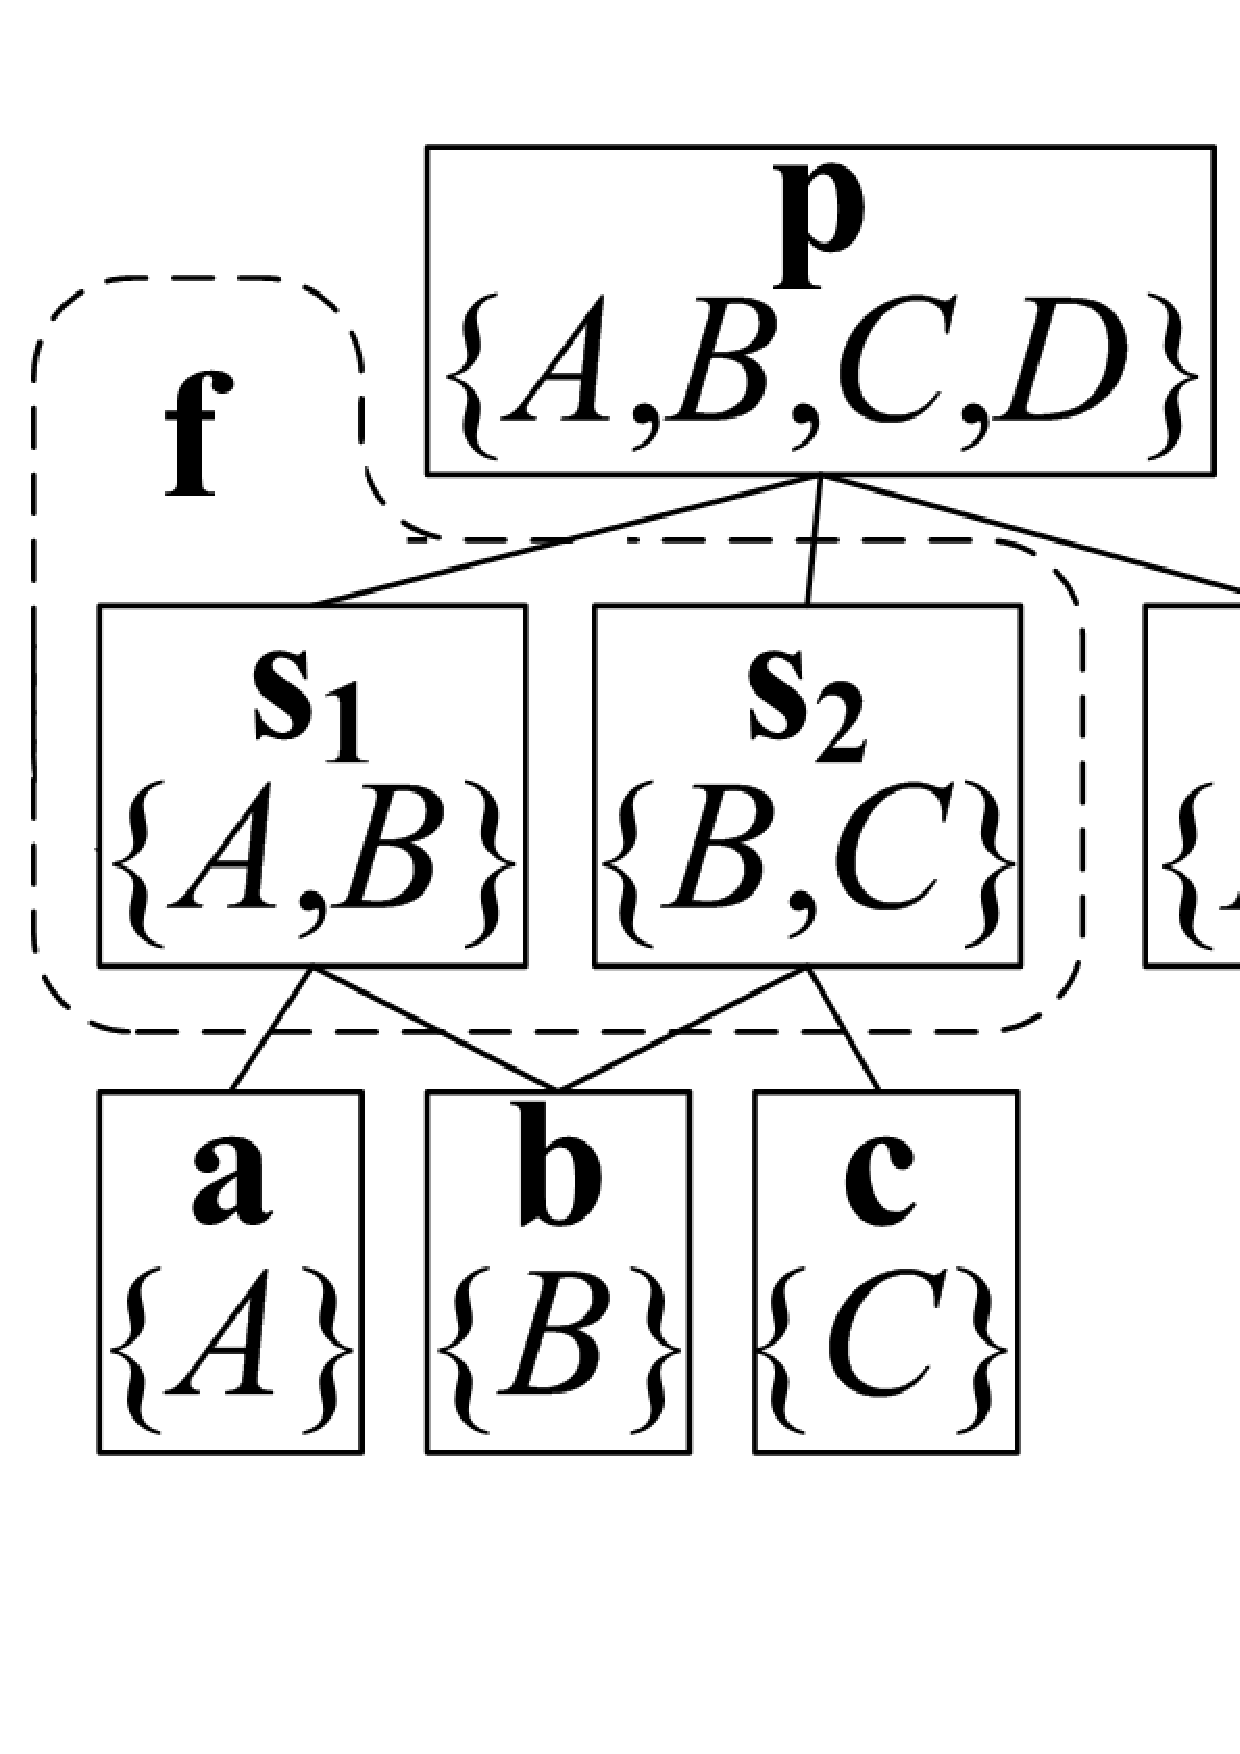
\includegraphics[scale=1.0]{images/gg_algo_class.png}
\caption{Пример части диаграммы Хассе, обрабатываемой алгоритмом \ref{alg:build_gg}.}
\label{fig:gg_algo_example}
\end{minipage}
\hspace{0.5cm}
\begin{minipage}[t]{0.4\textwidth}
\centering
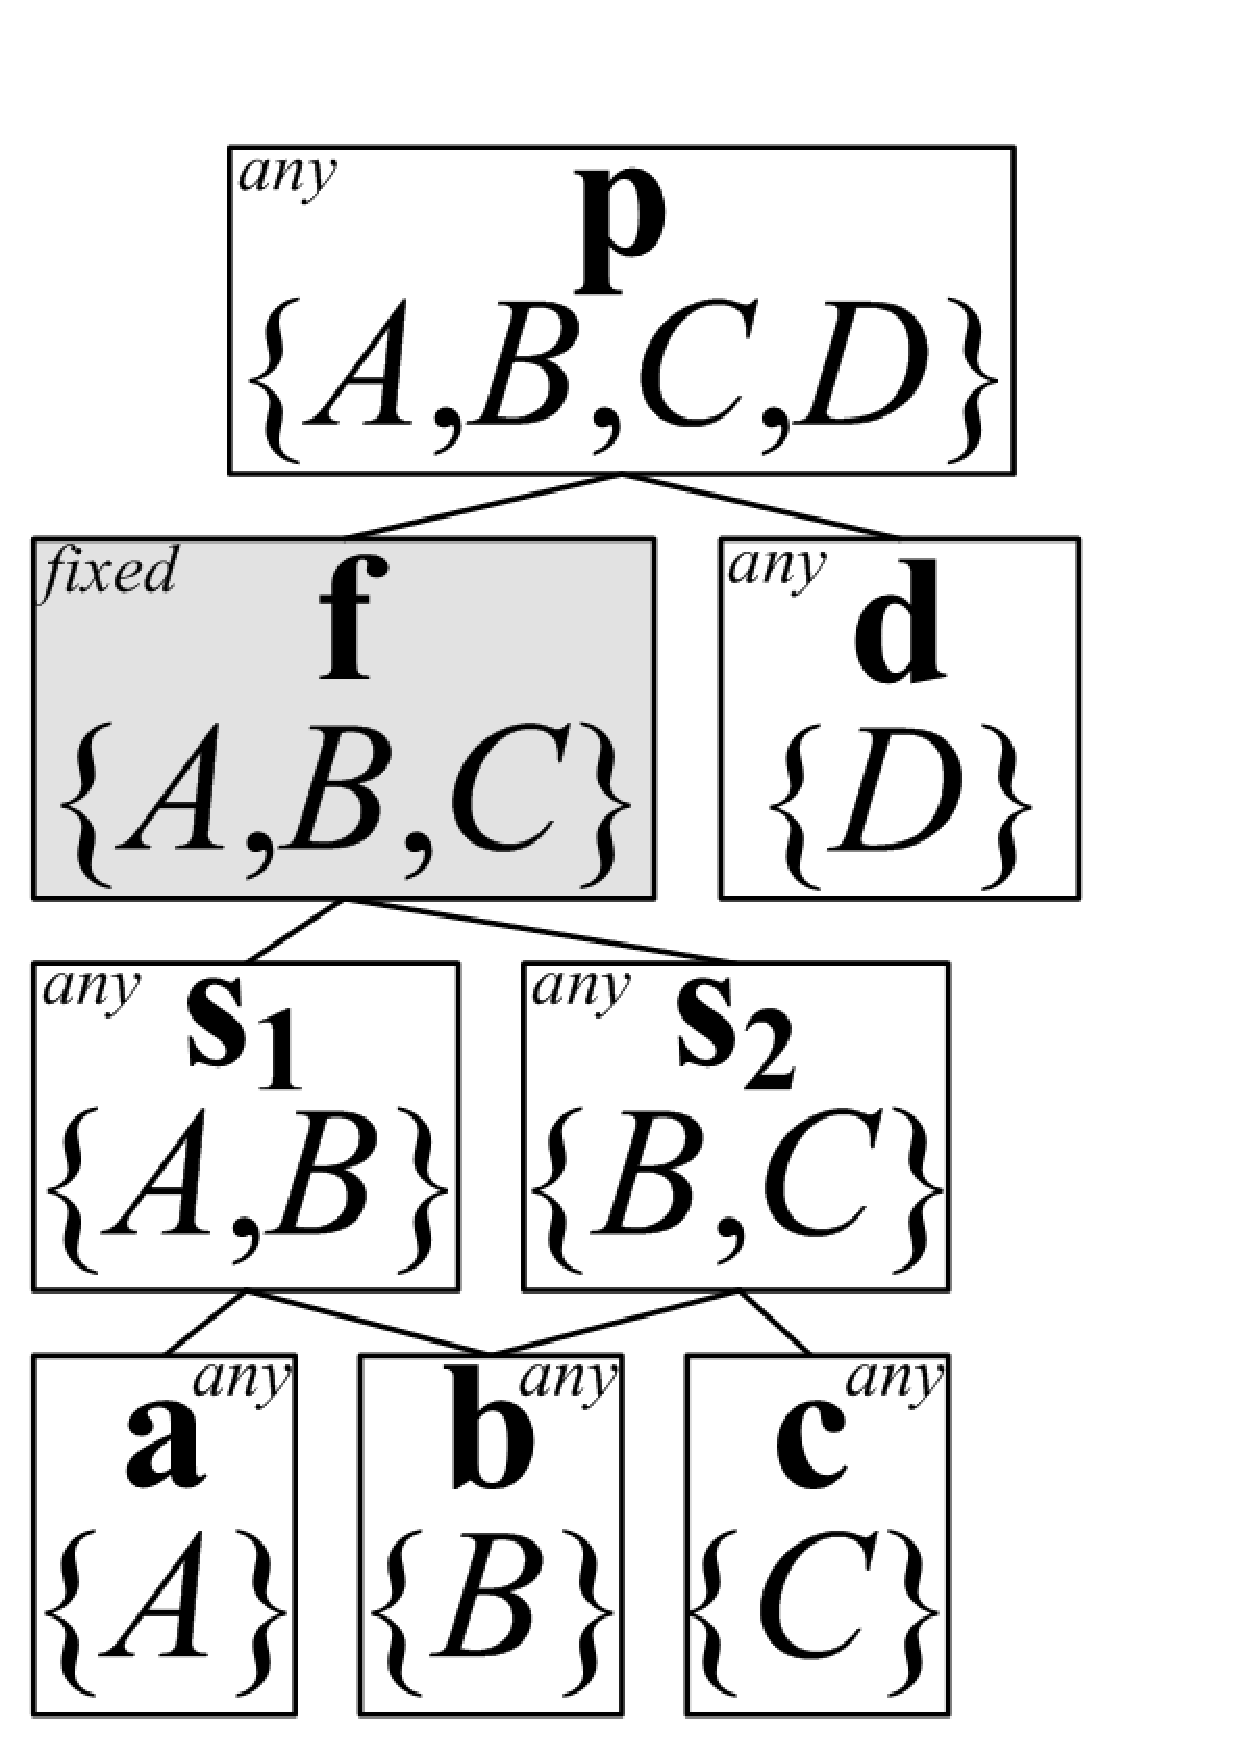
\includegraphics[scale=1.0]{images/gg_algo_class_2.png}
\caption{Результат обработки алгоритмом \ref{alg:build_gg} части диаграммы Хассе, представленной на рис. \ref{fig:gg_algo_example}.}
\label{fig:gg_algo_result}
\end{minipage}
\end{figure}

Пример работы алгоритма \ref{alg:build_gg} приведен на рис. \ref{fig:gg_algo_example} и рис. \ref{fig:gg_algo_result}. На рис. \ref{fig:gg_algo_example} представлена часть исходной диаграммы Хассе $\gH$, а на рис. \ref{fig:gg_algo_result} --- соответствующая ей часть графа $\gG$. Так как вершины $\gf_1$ и $\gf_2$ диаграммы Хассе $\gH$ лежат в одном множестве $\gf'_1 \in \gK$, то для них была добавлена $\fixed$-вершина $\gf'_1$. Для вершины же $\gf_3$ выполнено $\gf_3 = \gf'_2$, и потому $\gf'_2 \in \gD$, и для $\gf_3$ дополнительных $\fixed$-вершин добавлено не было.

По построению, граф $\gG$ является диаграммой Хассе для множества, подмножеством которого является $\gFs$, и потому на $\gG$ определен порядок расположения вершин на плоскости, и аналогично $\gH$ для каждой вершины определено множество дочерних вершин. Также по построению каждой $\any$-вершине в $\gG$ соответствует вершина в $\gH$, и наоборот. Тогда, согласно теореме \ref{theorem:evil}, выбирая для каждой $\any$-вершины дерево на множестве ее дочерних вершин, и добавляя после этого ребра к дереву $T \in \nT(\gCa)$ так, как в алгоритме \ref{alg:build_tree}, можно получить произвольное дерево, являющееся частичным решением задачи \ref{eq:problem}.

%Согласно утверждениям \ref{stmt:fsets_2}

С помощью графа $\gG$ построим полное решение задачи \ref{eq:relaxed_problem}.

%Для построения полного решения достаточно для каждого ребра построенного дерева $T$ определить направление наследование на этом ребре так, чтобы для каждой вершины дерева, то есть класса, существовал ровно один непосредственный базовый класс в этом дереве.

Заметим, что в графе $\gG$ нет циклов, проходящих только по $\any$-вершинам --- для существования цикла, проходящего через вершину $\gf$, и две ее дочерние вершины $\gf_1$ и $\gf_2$ необходимо, чтобы в $\gH$ существовал путь между вершинами $\gf_1$ и $\gf_2$. Но существование такого пути означает, что пересечение множеств $\gf_1$ и $\gf_2$ не пусто, и потому на этапе построения графа $\gG$ две эти вершины были отнесены к одному множеству $\gf'_1$, как это показано на рис. \ref{fig:gg_algo_example}. Следовательно, для этих вершин была добавлена $\fixed$-вершина, как это показано на рис. \ref{fig:gg_algo_result}, и потому они не могут являться дочерними для $\gf$. Это означает, что невозможно появление цикла, проходящего только по $\any$-вершинам, и содержащего вершины $\gf$, $\gf_1$ и $\gf_2$. Также для каждой $\any$-вершины $\gf$ графа $\gG$ выполнено:
\begin{equation}\label{eq:number_of_children}
|\children(\gf)| \le |\gCa| \text{,}
\end{equation}
то есть $\gf$ имеет не более $|\gCa|$ дочерних вершин. Если бы $\any$-вершина $\gf$ имела более $|\gCa|$ дочерних вершин, то пересечение некоторых двух из них было бы не пусто, что, как было только что доказано, невозможно.

Определим несколько функций. Пусть:

{\centering
\begin{tabularx}{\textwidth}{rcX}
    $\type$ & --- & возвращает тип данной вершины, то есть значение из множества $\{\any, \fixed\}$; \\
   $\class$ & --- & если для данной вершины $\gf$ выполнено $|\gf| = 1$, то есть $\gf = \{C\}$, то возвращает $C$, иначе возвращает $\emptyset$; \\
$\adjacent$ & --- & для данной вершины возвращает множество смежных с ней вершин в графе $\gG$; \\
 $\parents$ & --- & для данной вершины $\gf$ возвращает множество вершин, для которых $\gf$ является дочерней в $\gG$, то есть $\parents(\gf) = \adjacent(\gf) \setminus \children(\gf)$. По построению, если $\type(\gf) = \fixed$, то в этом множестве содержится ровно одна вершина. \\
\end{tabularx}}

Всевозможным парам вершин $(\gf_1, \gf_2)$ графа $\gG$ поставим в соответствие множества достижимых из $\gf_1$ по направлению на $\gf_2$ классов $\gC_{(\gf_1, \gf_2)}$. Если две вершины $\gf_1$ и $\gf_2$ инцидентны в графе $\gG$, то $\gC_{(\gf_1, \gf_2)}$ для них определяется согласно следующим правилам:
\begin{equation}\label{eq:cset_for_class}
\type(\gf_1) = \type(\gf_2) = \any \wedge \class(\gf_2) \ne \emptyset \Longrightarrow \gC_{(\gf_1, \gf_2)} = \class(\gf_2) \text{,}
\end{equation}

Иначе, если выполнено:
\begin{equation}\label{eq:cset_for_rest_cond}
\begin{aligned}
&\left( \type(\gf_1) = \type(\gf_2) = \any \right) \vee \\
&\left( \exists \{\gf'_1, \gf'_2\} = \{\gf_1, \gf_2\}: \type(\gf'_1) = \any \wedge \type(\gf'_2) = \fixed \wedge \parents(\gf'_2) = \{\gf'_1\} \right) \text{,}
\end{aligned}
\end{equation}
то есть $\gf_1$ и $\gf_2$ являются $\any$-вершинами, или одна из вершин $\gf_1$ и $\gf_2$ является $\fixed$-вершиной, а другая --- $\any$-вершиной, причем $\fixed$-вершина является дочерней для $\any$-вершины, то:
\begin{equation}\label{eq:cset_for_rest}
\gC_{(\gf_1, \gf_2)} = \bigcup_{\gf \in \adjacent(\gf_2) \setminus \gf_1} \gC_{(\gf_2, \gf)} \text{.}
\end{equation}

В случае, если не выполнено ни (\ref{eq:cset_for_class}), ни (\ref{eq:cset_for_rest_cond}), множество $\gC_{(\gf_1, \gf_2)}$ пусто.

Так как для двух вершин $\gf_1$ и $\gf_2$ таких, что $\gf_1$ является $\fixed$-вершиной, $\gf_2$ --- $\any$-вершиной, и $\gf_2$ является дочерней для $\gf_1$, множество $\gC_{(\gf_1, \gf_2)}$ пусто, то в силу отсутствия циклов в графе $\gG$, проходящих только по $\any$-вершинам, рекурсивное определение (\ref{eq:cset_for_rest}) множества $\gC_{(\gf_1, \gf_2)}$ корректно.

%Ребра графа $\gG$, инцидентные двум вершинам $\gf_1$ и $\gf_2$, для которых построенные с использованием правил (\ref{eq:cset_for_class})-(\ref{eq:cset_for_rest}) множества $\gC_{(\gf_1, \gf_2)}$ и $\gC_{(\gf_2, \gf_1)}$ не пусты, обозначим $\gE$.

Изменим множества $\gC_{(\gf_1, \gf_2)}$ для таких пар вершин, что $\gf_1$ является $\any$-вершиной, $\gf_2$ --- $\fixed$-вершиной, и между $\gf_2$ и $\gf_1$ в $\gG$ существует путь, содержащий только одну $\fixed$-вершину $\gf_2$, и такой, что каждая вершина в этом пути является дочерней для предыдущей. Это означает, что $\gf_2$ является <<первой>> $\fixed$-вершиной, находящейся над $\gf_1$, и связанной с ней. В этом случае будем считать, что
\begin{equation}
\gC_{(\gf_1, \gf_2)} = \gCa \setminus \left( \class(\gf_1) \cup \bigcup_{\gf \in \gCa} \gC_{(\gf_1, \gf)} \right)
\end{equation}
Тогда для каждой вершины $\gf$, по построению выполнено:
\begin{equation}\label{eq:gc_props}
\begin{aligned}
&\bigcup_{\gf' \in \gG_V} \gC_{(\gf, \gf')} = \gCa \setminus \class(\gf) \text{,} \\
&\forall_{\gf_1, \gf_2 \in \gG_V} \gC_{(\gf, \gf_1)} \cap \gC_{(\gf, \gf_2)} = \emptyset \text{.}
\end{aligned}
\end{equation}

Будем строить дерево, являющееся решением задачи (\ref{eq:relaxed_problem}) как дерево $T \in \nT(\gCa)$, для каждого ребра которого определено направление наследования. Для этого:
\begin{enumerate}
\item Для каждых двух дочерних вершин $\gf_1$ и $\gf_2$ каждой $\any$-вершины $\gf$ построим множество $\gN^{\gf}_{(\gf_1, \gf_2)}$ --- множество классов, которые должен унаследовать корень $T[\gf_1]$ в случае, если существует класс в $\gf_2$, являющийся предком этого корня, и множество $\gP^{\gf}_{(\gf_1, \gf_2)}$ --- множество классов, которые корень $T[\gf_1]$ не должен унаследовать в том же случае.
\item Для каждой $\any$-вершины $\gf$ построим корневое дерево $T_{\gf} \in \nT(\children(\gf))$ на множестве дочерних для нее вершин в $\gG$.
\end{enumerate}
Согласно определению, для множеств $\gN^{\gf}_{(\gf_1, \gf_2)}$ и $\gP^{\gf}_{(\gf_1, \gf_2)}$ выполнено:
\begin{equation}\label{eq:gn_gp_in_gc}
\gP^{\gf}_{(\gf_1, \gf_2)}, \gN^{\gf}_{(\gf_1, \gf_2)} \subseteq \gC_{(\gf_1, \gf_2)}
\end{equation}

Для построения корневых деревьев $T_{\gf}$ в каждой $\any$-вершине будем восстанавливать отношение $\lhd$ на множестве дочерних для нее вершин. Отношение $\lhd$ для вершины $\gf$ будем задавать множеством ограничений $\gR_{\gf}$. Будем считать, что в процессе восстановления это отношение задано ограничениями следующего вида:
\begin{equation}\label{eq:restriction_type}
\begin{aligned}
\cR &= B < D \text{,} &\text{или} \\
\cR &= B \lhd D \text{,} &\text{или} \\
\cR &= A \sim C \text{.} &~
\end{aligned}
\end{equation}
Ограничения вида $\cR = \neg (A \sim C)$ можно заменить двумя ограничениями $\cR_1 = A < C$ и $\cR_2 = A > C$ и рассматривать как ограничения вида (\ref{eq:restriction_type}).

Все ограничения из $\gR$, за исключением ограничений вида $\cR_{\ref{stmt:fsets_2}}$, полученных применением утверждения \ref{stmt:fsets_2}, представимы в виде \ref{eq:restriction_type}. Согласно предположению, высказанному в конце главы \ref{chapter:part_single_inher_rec}, все ограничения вида $\cR_{\ref{stmt:fsets_2}}$ выполнимы, и согласно теореме \ref{theorem:evil}, любое дерево, построенное с помощью алгоритма \ref{alg:build_tree}, удовлетворяет этим ограничениям. Тогда соблюдение ограничений вида $\cR_{\ref{stmt:fsets_2}}$ обеспечивается структурой построенного графа $\gG$ и выбранным способом построения корневого дерева, являющегося решением задачи (\ref{eq:relaxed_problem}).

Пусть $\gR_s \subseteq \gR$ --- множество всех ограничений из $\gR$, представимых в виде (\ref{eq:restriction_type}). Тогда в $\gR_s$ содержатся все ограничения из $\gR$, кроме ограничений вида $\cR_{\ref{stmt:fsets_2}}$. В начале главы \ref{chapter:full_sing_inhr_rec} было отмечено, что некоторые из ограничений из $\gR$ могут оказаться ложными, и вызвать конфликты в ходе восстановления иерархии. Будем строить иерархию, рассматривая ограничения из $\gR_s$ в порядке увеличения вероятности получения конфликта. Ограничения вида $\cR_{\ref{stmt:destructors}}$, определенные в утверждении \ref{stmt:destructors}, всегда выполняются, и являются наиболее информативными. В результате проведения экспериментов было выяснено, что во многих случаях только ограничений вида $\cR_{\ref{stmt:destructors}}$ и $\cR_{\ref{stmt:fsets_2}}$ достаточно, чтобы полностью восстановить иерархию классов. Поэтому будем рассматривать ограничения начиная с ограничений вида $\cR_{\ref{stmt:destructors}}$. В случае, если на очередном шаге обнаружится конфликт в структуре построенных множеств, в результате чего построение корневого дерева, являющегося решением, станет невозможным, будем возвращаться к предыдущему шагу, и продолжить обработку, добавив ограничение, вызвавшее конфликт, в изначально пустое множество конфликтных ограничений $\gR_{\times}$. Тогда после завершения обработки всех ограничений из $\gR_s$, множество ограничений $\gR \setminus \gR_{\times}$ будет соответствовать множеству ограничений $\gR'$ из определения задачи (\ref{eq:relaxed_problem}).


\begin{figure}[htb!]
\begin{algorithmic}[1]
\STATE \textbf{let} $\cR \in \gR_s, A, C \in \gCa: A \ne C \wedge \cR = A \sim C$
\STATE \textbf{let} $\gf_1: \class(\gf_1) = \{C\}$
\WHILE{$\class(\gf_1) \ne \{A\}$}
    \STATE \COMMENT{$\gf_2$ существует и единственно в силу (\ref{eq:gc_props})}
    \STATE \textbf{let} $\gf_2 \in \adjacent(\gf_1): A \in \gC_{(\gf_1, \gf_2)}$
    \IF{$\type(\gf_2) = \any \wedge \gf_1 \in \children(\gf_2) \wedge \exists \gf_3 \in \children(\gf_2): B \in \gC_{(\gf_2, \gf_3)}$}
%        \IF{$(\gf_1 \rhd \gf_3) \in \gR_{\gf_2}$}
%            \STATE $\gR_s \gets \gR_s \cup \{A \rhd C\}$
%        \ELSIF{$(\gf_3 \rhd \gf_1) \in \gR_{\gf_2}$}
%            \STATE $\gR_s \gets \gR_s \cup \{C \rhd A\}$
%        \ENDIF
%        \STATE $\gR_{\gf_2} \gets \gR_{\gf_2} \cup \{\gf_1 \sim \gf_3\}$
        \STATE $\gN^{\gf_2}_{(\gf_1, \gf_3)} \gets \gN^{\gf_2}_{(\gf_1, \gf_3)} \cup \{C\}$
        \STATE $\gN^{\gf_2}_{(\gf_3, \gf_1)} \gets \gN^{\gf_2}_{(\gf_3, \gf_1)} \cup \{A\}$
    \ELSIF{$\type(\gf_2) = \fixed \wedge \gf_2 \in \children(\gf_1)$}
        \STATE \textbf{break}
    \ENDIF
    \STATE $\gf_1 \gets \gf_2$
\ENDWHILE
\end{algorithmic}
\caption{Алгоритм обработки ограничения вида  $A \sim C$.}
\label{alg:process_sim}
\end{figure}

\begin{figure}[htb!]
\begin{algorithmic}[1]
\STATE \textbf{let} $\cR \in \gR_s, B, D \in \gCa: B \ne C \wedge \cR = B < D$
\STATE \textbf{let} $\gf_1: \class(\gf_1) = \{D\}$
\WHILE{$\class(\gf_1) \ne \{B\}$}
    \STATE \COMMENT{$\gf_2$ существует и единственно в силу (\ref{eq:gc_props})}
    \STATE \textbf{let} $\gf_2 \in \adjacent(\gf_1): B \in \gC_{(\gf_1, \gf_2)}$
    \IF{$\type(\gf_2) = \any \wedge \gf_1 \in \children(\gf_2) \wedge \exists \gf_3 \in \children(\gf_2): B \in \gC_{(\gf_2, \gf_3)}$}
        \STATE $\gN^{\gf_2}_{(\gf_1, \gf_3)} \gets \gN^{\gf_2}_{(\gf_1, \gf_3)} \cup \{B\}$
        \STATE $\gP^{\gf_2}_{(\gf_3, \gf_1)} \gets \gP^{\gf_2}_{(\gf_3, \gf_1)} \cup \{D\}$
    \ELSIF{$\type(\gf_2) = \fixed \wedge \gf_2 \in \children(\gf_1)$}
        \STATE \textbf{break}
    \ENDIF
    \STATE $\gf_1 \gets \gf_2$
\ENDWHILE
\end{algorithmic}
\caption{Алгоритм обработки ограничения вида $B < D$.}
\label{alg:process_less}
\end{figure}

\if 0
\begin{figure}[htb!]
\begin{algorithmic}[1]
\STATE \textbf{let} $\cR \in \gR_s: \cR = B \lhd D$
\STATE \textbf{let} $\gf_1: \class(\gf_1) = \{D\}$
\WHILE{$\class(\gf_1) \ne \{B\}$}
    \STATE \COMMENT{$\gf_2$ существует и единственно в силу (\ref{eq:gc_props})}
    \STATE \textbf{let} $\gf_2 \in \adjacent(\gf_1): B \in \gC_{(\gf_1, \gf_2)}$
    \IF{$\type(\gf_2) = \any \wedge \gf_1 \in \children(\gf_2) \wedge \exists \gf_3 \in \children(\gf_2): B \in \gC_{(\gf_2, \gf_3)}$}
        \STATE $\gR_{\gf_2} \gets \gR_{\gf_2} \cup \{\gf_1 \rhd \gf_3\}$
        \STATE $\gN^{\gf_2}_{(\gf_1, \gf_3)} \gets \gN^{\gf_2}_{(\gf_1, \gf_3)} \cup \{B\}$
    \ELSIF{$\type(\gf_2) = \fixed \wedge \gf_2 \in \children(\gf_1)$}
        \STATE \textbf{break}
    \ENDIF
    \STATE $\gf_1 \gets \gf_2$
\ENDWHILE
\end{algorithmic}
\caption{Алгоритм обработки ограничения вида $B \lhd D$.}
\label{alg:process_lhd}
\end{figure}
\fi

Будем считать, что изначально множества ограничений $\gR_{\gf}$, а также множества $\gN^{\gf}_{(\gf_1, \gf_2)}$ и $\gP^{\gf}_{(\gf_1, \gf_2)}$ пусты. Сначала рассмотрим все ограничения $\cR_{\ref{stmt:destructors}}$, затем --- все прочие ограничения вида $B \lhd D$. Так как отношение $\lhd$ можно выразить через отношения $<$ и $\sim$, то приведем алгоритмы модификации множеств $\gN^{\gf}_{(\gf_1, \gf_2)}$, $\gP^{\gf}_{(\gf_1, \gf_2)}$ и $\gR_{\gf}$ только для ограничений вида $B < D$ и $A \sim C$. Алгоритм отработки отдельного ограничения вида $A \sim C$ представлен на рис. \ref{alg:process_sim}, а ограничения вида $B < D$ --- на рис. \ref{alg:process_less}.

%Алгоритм модификации множеств $\gN^{\gf}_{(\gf_1, \gf_2)}$, $\gP^{\gf}_{(\gf_1, \gf_2)}$ и $\gR_{\gf}$ для отдельного ограничения такого вида представлен на рис. \ref{alg:process_lhd}.

После работы этих алгоритмов из измененных множеств $\gN^{\gf}_{(\gf_2, \gf_1)}$ и $\gP^{\gf}_{(\gf_1, \gf_2)}$ можно извлечь дополнительную информацию об ограничениях из $\gR_{\gf}$ с использованием правил поддержания непротиворечивости для множеств $\gR_{\gf}$. Из определения множеств $\gN^{\gf}_{(\gf_1, \gf_2)}$ и отношения $\sim$ следует:
\begin{equation}\label{eq:gf_consistency_1}
\begin{aligned}
&\forall \gf \in \gG_V: \type(\gf) = \any, \gf_1, \gf_2 \in \children(\gf): \gN^{\gf}_{(\gf_1, \gf_2)} \ne \emptyset \wedge \gN^{\gf}_{(\gf_2, \gf_1)} \ne \emptyset \\
&\quad \Longrightarrow (\gf_1 \sim \gf_2) \in \gR_{\gf}
\end{aligned}
\end{equation}

Множества $\gP^{\gf}_{(\gf_1, \gf_2)}$ и $\gN^{\gf}_{(\gf_1, \gf_2)}$ не должны конфликтовать, то есть должно быть выполнено:
\begin{equation}\label{eq:gf_consistency_2}
\begin{aligned}
&\forall \gf \in \gG_V: \type(\gf) = \any, \gf_1, \gf_2 \in \children(\gf): \gP^{\gf}_{(\gf_1, \gf_2)} \cap \gN^{\gf}_{(\gf_1, \gf_2)} \ne \emptyset \\
&\quad \Longrightarrow (\gf_1 < \gf_2) \in \gR_{\gf}
\end{aligned}
\end{equation}

Отношение $\lhd$ транзитивно, и потому выполнено:
\begin{equation}\label{eq:gf_consistency_3}
\begin{aligned}
&\exists \gf \in \gG_V: \type(\gf) = \any, \gf_1, \gf_2, \gf_3 \in \children(\gf): \{\gf_1 \rhd \gf_2, \gf_2 \rhd \gf_3\} \subseteq \gR_{\gf} \\
&\quad \Longrightarrow (\gf_1 \rhd \gf_3) \in \gR_{\gf} %\wedge \gN^{\gf}_{(\gf_2, \gf_3)} \subseteq \gN^{\gf}_{(\gf_1, \gf_3)}
\end{aligned}
\end{equation}

После применения правил поддержания непротиворечивости (\ref{eq:gf_consistency_1}), (\ref{eq:gf_consistency_2}) и (\ref{eq:gf_consistency_3}) в множества $\gR_{\gf}$ могут быть добавлены новые ограничения. Для элементов этих множеств используются следующие правила поддержания непротиворечивости:
\begin{equation}\label{eq:consistency_gr}
\begin{aligned}
b \lhd d &\Longleftrightarrow b < d \wedge b \sim d \\
b \lhd c \wedge c \lhd d &\Longrightarrow b \lhd d \\
d_1 \sim d_2, \ldots, d_{n - 1} \sim d_n, d_n \sim d_1\} &\Longrightarrow \forall a, c \in \{d_1, \ldots, d_n\}: a \sim c
\end{aligned}
\end{equation}
Эти правила опираются на свойства отношений $<$, $\lhd$ и $\sim$, а также на то, что эти отношения должны задавать деревья на множествах $\children(\gf)$. Также во множествах $\gR_{\gf}$ не должно существовать конфликтов, то есть не должно быть выполнено:
\begin{equation}\label{eq:consistency_conflict_1}
b \sim d \wedge b > d \wedge b < d
\end{equation}

Из измененных множеств $\gR_{\gf}$ может быть извлечена дополнительная информация об отношении наследования на множестве $\gCa$ с использованием правил поддержания непротиворечивости для множества $\gCa$. По одному ребру в дереве наследования не может быть унаследовано два класса, не связанных наследованием, и потому выполнено:
\begin{equation}\label{eq:gca_consistency_1}
\begin{aligned}
&\exists \gf \in \gG_V: \type(\gf) = \any, \gf_1, \gf_2 \in \children(\gf): \{\gf_1 \rhd \gf_2\} \subseteq \gR_{\gf}, A, C \in \gN^{\gf}_{(\gf_1, \gf_2)}: A \ne C \\
&\quad \Longrightarrow \text{~выполнено~} A \sim C
\end{aligned}
\end{equation}

В силу того, что в $\gG$ не существует цикла, проходящего только по $\any$-вершинам, выполнено:
\begin{equation}\label{eq:gca_consistency_2}
\begin{aligned}
&\exists \gf \in \gG_V: \type(\gf) = \any, \gf_1, \gf_2 \in \children(\gf): \{\gf_1 \rhd \gf_2\} \subseteq \gR_{\gf}, B \in \gN^{\gf}_{(\gf_1, \gf_2)} \\
&\quad \Longrightarrow \forall D \in \gC_{(\gf, \gf_1)}: \text{~выполнено~} D \rhd B
\end{aligned}
\end{equation}

\begin{equation}\label{eq:gca_consistency_3}
\begin{aligned}
&\exists \gf \in \gG_V: \type(\gf) = \any, \gf_1, \gf_2 \in \children(\gf): \{\gf_1 \rhd \gf_2\} \subseteq \gR_{\gf}, B \in \gN^{\gf}_{(\gf_1, \gf_2)} \\
&\quad \Longrightarrow \forall D \in \gP_{(\gf_1, \gf_2)}: \text{~выполнено~} D > B
\end{aligned}
\end{equation}

Таким образом, применение алгоритмов \ref{alg:process_sim} и \ref{alg:process_less} добавляет новые элементы в множества $\gN^{\gf}_{(\gf_2, \gf_1)}$ и $\gP^{\gf}_{(\gf_1, \gf_2)}$, применение правил поддержания непротиворечивости (\ref{eq:gf_consistency_1}), (\ref{eq:gf_consistency_2}) и (\ref{eq:gf_consistency_3}) на основе добавленных элементов добавляет ограничения в множества $\gR_{\gf}$, применение правил (\ref{eq:consistency_gr}) также добавляет новые ограничения в множества $\gR_{\gf}$, а применение правил поддержания непротиворечивости (\ref{eq:gca_consistency_1}) и (\ref{eq:gca_consistency_3}) добавляет новые ограничения на классы из $\gCa$, к которым снова можно применить алгоритмы \ref{alg:process_sim} и \ref{alg:process_less}. Так как все рассматриваемые множества конечны, то такой цикл применения алгоритмов \ref{alg:process_sim} и \ref{alg:process_less} и правил поддержания непротиворечивости (\ref{eq:gf_consistency_1}), (\ref{eq:gf_consistency_2}), (\ref{eq:gf_consistency_3}), (\ref{eq:consistency_gr}), (\ref{eq:gca_consistency_1}) и (\ref{eq:gca_consistency_3}) не может быть бесконечен. Этот цикл необходимо применить к каждому из ограничений из $\gR_s$.

Если в результате применения цикла к очередному ограничению $\cR$ из множества $\gR_s$ было нарушено (\ref{eq:consistency_conflict_1}) в одном из множеств $\gR_{\gf}$, или выяснилось, что не существует корневого дерева $T_{\gf} \in \nT^R(\children(\gf))$, удовлетворяющего ограничениям $\gR_{\gf}$, или (\ref{eq:consistency_conflict_1}) было нарушено для восстанавливаемого отношения наследования на множестве $\gCa$, то следует вернуться к предыдущему шагу, добавив ограничение $\cR$ в множество конфликтных ограничений $\gR_{\times}$.

%Количество ограничений в множестве $\gR_s$ конечно, и потому алгоритм завершится.

%Также в силу определения множеств $\gN^{\gf}_{(\gf_1, \gf_2)}$ должно быть выполнено:
%\begin{equation}\label{eq:consistency_4}
%\begin{aligned}
%&\exists \gf \in \gG_V: \type(\gf) = \any, \gf_1, \gf_2 \in \children(\gf), A \in \gN^{\gf}_{(\gf_1, \gf_2)}, C \in \gN^{\gf}_{(\gf_2, \gf_1)}: A \ne C \\
%&\quad \Longrightarrow \text{~выполнено~} A \sim C
%\end{aligned}
%\end{equation}

%Существование решения также требует:
%\begin{equation}\label{eq:consistency_6}
%\begin{aligned}
%&\exists \gf \in \gG_V: \type(\gf) = \any, \gf_1, \gf_2 \in \children(\gf): (\gf_1 \rhd \gf_2) \in \gR_{\gf}, B \in \gN^{\gf}_{(\gf_1, \gf_2)}, C \in \gP^{\gf_2}_{(\gf_3, \gf_1)} \\
%&\quad \Longrightarrow \text{~выполнено~} B < C
%\end{aligned}
%\end{equation}

%Если после обработки очередного ограничения возникает конфликт в (\ref{eq:consistency_conflict_1}), то следует вернуться к предыдущему шагу, и продолжить обработку прочих ограничений. Обработав все ограничения $B \lhd D$, перейдем к ограничениям $\cR = A \sim C$. Алгоритм обработки отдельного ограничения такого вида представлен на рис. \ref{alg:process_sim}.

%После работы этого алгоритма в множество $\gR_s$ могли быть добавлены новые ограничения вида $B \lhd D$. Их следует обработать в первую очередь. На следующем шаге следует обработать ограничения $B < D$. Алгоритм обработки ограничений такого вида представлен на рис. \ref{alg:process_less}.

%Этот алгоритм модифицирует множества $\gP^{\gf_2}_{(\gf_3, \gf_1)}$, для которых также должны быть выполнены правила консистентности. В силу транзитивности $\lhd$ должно быть выполнено:
%\begin{equation}\label{eq:consistency_5}
%\begin{aligned}
%&\exists \gf \in \gG_V: \type(\gf) = \any, \gf_1, \gf_2, \gf_3 \in \children(\gf): \{\gf_1 \rhd \gf_2, \gf_2 \rhd \gf_3\} \subseteq \gR_{\gf} \\
%&\quad \Longrightarrow \gP^{\gf}_{(\gf_1, \gf_3)} \subseteq \gP^{\gf}_{(\gf_2, \gf_3)}
%\end{aligned}
%\end{equation}

%Для множеств ограничений $\gR_{\gf}$ также должно использоваться правило поддержания консистентности (\ref{eq:consistency_gr}) и не должно существовать конфликтов вида (\ref{eq:consistency_conflict_1}), а также на каждом шаге должно быть возможно построить корневое дерево $T_{\gf} \in \nT^R(\children(\gf))$, удовлетворяющее ограничениям $\gR_{\gf}$. Если после обработки очередного ограничения возникает конфликт в (\ref{eq:consistency_conflict_1}), то следует вернуться к предыдущему шагу, и продолжить обработку прочих ограничений.

Обработав все ограничения, построим дерево $T$. Для этого для каждой $\any$-вершины $\gf$ построим корневое дерево $T_{\gf} \in \nT^R(\children(\gf))$ на множестве дочерних для нее вершин в $\gG$. По построению такое дерево существует. Будем рассматривать $\any$-вершины из $\gG$ в порядке снизу вверх и строить для них соответствующие деревья $T[\gf]$. Пусть $\gf$ --- очередная такая вершина, и для всех ее дочерних вершин соответствующие деревья уже построены, то есть $\forall \gf' \in \children(\gf): T[\gf'] \in \nT^R(\gf')$. Будем рассматривать такие деревья как ориентированные графы, в которых все дуги имеют направление от листьев к корню дерева. Для каждой дуги $(\gf_1, \gf_2)$ из $T_{\gf}$ добавим в $T$ дугу, соединяющую корень $T[\gf_1]$, и вершину из $\gf_2$ такую, что по дугам достижимы все вершины из $\gN^{\gf}_{(\gf_1, \gf_2)}$, и не достижимы вершины из $\gP^{\gf_2}_{(\gf_3, \gf_1)}$. Существование такой вершины следует из выполнения (\ref{eq:gca_consistency_3}). Добавив все такие дуги, выберем корень дерева $T[\gf_r]$ корнем построенного дерева $T[\gf]$, где $\gf_r$ --- корень $T_{\gf}$. Так как такое построение полностью соответствует описанному в алгоритме \ref{alg:build_tree}, то согласно теореме \ref{theorem:evil}, для построенного корневого дерева $T$ выполнены все ограничения, порожденные утверждением \ref{stmt:fsets_2}. По построению для этого дерева также выполнено множество ограничений $\gR \setminus \gR_{\times}$, и потому построенное дерево является решением задачи \ref{eq:relaxed_problem}.


Оценим сложность представленного алгоритма. Пусть $n$ --- количество классов в множестве $\gCa$. Как было отмечено в главе \ref{chapter:part_single_inher_rec}, в задачах, встречающихся на практике, размер множества $\gFc$ в большинстве случаев не превышает $n^2$. Пусть $N$ --- количество $\any$-вершин в графе $\gG$. Так как каждой $\any$-вершине графа $\gG$ соответствует элемент множества $\gFs$, то согласно (\ref{eq:gfs_def}), можно считать, что $N = O(n^2)$. Тогда в силу (\ref{eq:gc_props}), суммарный размер множеств $\gC_{(\gf_1, \gf_2)}$ не превосходит $nN$.

Дочерними вершинами $\any$-вершин могут быть другие $\any$-вершины, и $\fixed$-вершины. Так как в $\gG$ нет циклов, проходящих целиком по $\any$-вершинам, то количество ребер, соединяющих $\any$-вершины, не превосходит $N$. По построению графа $\gG$, у каждой $\fixed$-вершины есть дочерние вершины, причем дочерними вершинами $\fixed$-вершины могут быть только $\any$-вершины. Следовательно, в графе $\gG$ не более $N$ $\fixed$-вершин. Это в частности означает, что:
\begin{equation}\label{eq:vertices_in_ggv}
|\gG_V| \le 2N \text{.}
\end{equation}

Так как предком каждой $\fixed$-вершины является единственная $\any$-вершина, то суммарное количество дочерних вершин всех $\any$-вершин не превосходит $2N$, то есть:
\begin{equation}\label{eq:sum_children}
\sum_{\gf \in \gG_V: \type(\gf) = \any} |\children(\gf)| \le 2N \text{.}
\end{equation}

Тогда из (\ref{eq:vertices_in_ggv}) следует, что суммарный размер всех множеств, соответствующих вершинам графа $\gG$, не превосходит $2nN$. Из (\ref{eq:number_of_children}) и (\ref{eq:sum_children}) также следует, что суммарное количество ограничений в множествах $\gR_{\gf}$ не превосходит $6nN$. Также из (\ref{eq:gn_gp_in_gc}), (\ref{eq:gc_props}) и (\ref{eq:sum_children}) следует, что суммарный размер всех множеств $\gN^{\gf}_{(\gf_1, \gf_2)}$ и $\gP^{\gf}_{(\gf_1, \gf_2)}$ не превосходит $4Nn$. Число же различных ограничений на множестве $\gCa$ не превосходит $3n^2$.

Это означает, что затраты памяти предложенного алгоритма составляют $O(nN) = O(n^3)$. Оценим вычислительные затраты предложенного алгоритма. Проверка выполнения условий (\ref{eq:gf_consistency_1})-(\ref{eq:gca_consistency_3}) производится только в случае, если множество, для которого производится проверка, было изменено. В результате анализа проверок (\ref{eq:gf_consistency_1})-(\ref{eq:gca_consistency_3}) было выяснено, что для выполнения каждой их них требуется не более $O(n^2)$ операций. Так как в процессе работы алгоритма элементы только добавляются в множества $\gN^{\gf}_{(\gf_1, \gf_2)}$, $\gP^{\gf}_{(\gf_1, \gf_2)}$, $\gR_{\gf}$, и множество ограничений над $\gCa$, то проверки (\ref{eq:gf_consistency_1})-(\ref{eq:gca_consistency_3}) будут применены не более одного раза к каждому из элементов этих множеств. Следовательно, суммарная сложность предложенного алгоритма составляет $O(n^5)$.

Не смотря на высокую сложность, предложенный алгоритм применим для большинства возникающих на практике задач, связанных с восстановлением иерархий классов при отсутствии информации о типах времени выполнения. Это объясняется тем, что деревья наследования, состоящие более чем из 100 классов, встречаются в крупных библиотеках, таких как Qt \cite{qt} или MFC \cite{mfc}, которые в большинстве случаев используют ту или иную форму информации о типах времени выполнения, и поэтому для таких деревьев наследования применение предложенного алгоритма не требуется.



\subsection{Восстановление множественного наследования}
Как было сказано в главе \ref{chapter:multiple_inheritance}, так как большинство иерархий классов используют виртуальные деструкторы, то путем анализа деструкторов в большинстве случаев можно выявить использование множественного наследования и определить, какие таблицы виртуальных функций принадлежат одному и тому же классу. В главе \ref{chapter:restore_single_inheritance} был описан алгоритм восстановления отношения одиночного наследования на множестве таблиц виртуальных функций.

Результатом последовательного применения описанного в главе \ref{chapter:restore_single_inheritance} алгоритма  восстановления одиночного наследования на множестве таблиц виртуальных функций является одно или несколько деревьев наследования $T_1, \ldots, T_n$. Будем предполагать, что деревья наследования из $T_1, \ldots, T_n$ восстановлены корректно в смысле, определенном в главе \ref{chapter:problem}. Результатом анализа деструкторов на предмет использования множественного наследования является набор множеств таблиц виртуальных функций $\gv_1, \ldots, \gv_m$ такой, что все таблицы виртуальных функций, принадлежащие одному множеству, принадлежат одному классу. Тогда, каждое из множеств $\gv_i$ задает отдельный класс, использующий множественное наследование. Объединив для каждого из множеств $\gv_1, \ldots, \gv_m$ соответствующие вершины в деревьях $T_1, \ldots, T_n$, можно получить иерархию, учитывающую множественное наследование. При этом следует учитывать, что, вообще говоря, два множества $\gv_i$ и $\gv_j$ могут иметь непустое пересечение --- это будет означать, что классы, соответствующие $\gv_i$ и $\gv_j$, используют один и тот же деструктор, и разделяют некоторые из таблиц виртуальных функций. Тогда исходя из предположения о том, что деревья наследования $T_1, \ldots, T_n$ были восстановлены корректно, согласно правилам наследования Си++ \cite{cpp03}, отношение непосредственного наследования между таблицами виртуальных функций из $(\gv_i \cup \gv_j) \setminus (\gv_i \cap \gv_j)$ задает отношение непосредственного наследования между классами, соответствующими $\gv_i$ и $\gv_j$. Следовательно, можно заменить в соответствии с этим отношением непосредственного наследования каждую из вершин в деревьях $T_1, \ldots, T_n$, соответствующую таблицам виртуальных функций из $\gv_i \cap \gv_j$, на две, одна из которых будет соответствовать множеству $\gv_i$, а другая --- $\gv_j$, после чего произвести объединение вершин деревьев $T_1, \ldots, T_n$ также, как и в случае отсутствия пересечений между $\gv_i$ и $\gv_j$. Аналогично рассматривается случай существования более двух множеств из $\gv_1, \ldots, \gv_m$, имеющих непустое пересечение.

Таким образом, восстановив одиночное наследования на множестве таблиц виртуальных функций, и выяснив путем анализа деструкторов, какие таблицы виртуальных функций принадлежат одним и тем же классам, можно также восстановить множественное наследование. В главе \ref{chapter:multiple_inheritance} было также отмечено, что в случае отсутствия виртуальных деструкторов множественное наследование может быть заменено одиночным без нарушения корректности. Поэтому в предположении о том, что все деревья наследования $T_1, \ldots, T_n$ были восстановлены корректно, итоговая иерархия классов, учитывающая множественное наследование, также будет восстановлена корректно.

%Также в главе \ref{chapter:multiple_inheritance} было отмечено, что путем анализа виртуальных деструкторов можно также вычислить смещения экземпляров каждого из базовых классов в экземпляре производного класса, использующего множественное наследование.

%Согласно бинарному нитерфейсу приложений, использоемому компиляторами GCC и MSVC, при множественном наследовании с использованием виртуальных деструкторов невозможна ситуация, когда для одного базового класса была создана новая таблица виртуальных функций, а для другого была использована имеющаяся \cite{gray94, gccabi}. Следовательно, каждая таблица виртуальных функций соответсвует только одному классу, использующему множественное наследование. Это соотвествие восстанавливается путем анализа виртуальных деструкторов --- если две таблицы виртуальных функций принадлежат одному и тому же классу, использующему множественное наследование, то эти таблицы разделяют один и тот же виртуальный деструктор.



































